\documentclass[fleqn,12pt]{article}
\usepackage[top=2cm, left=2cm,right=3cm,bottom=2cm]{geometry}
%\usepackage[fleqn]{amsmath}
\usepackage{amsmath}
\usepackage{url,enumerate}
\usepackage{ifthen}
\newboolean{answers}
\setboolean{answers}{true}  % set to true to include TODO statements
%\setboolean{answers}{false}  % set to false to use input statements
\usepackage{amssymb}
\usepackage{tikz}
\newcommand{\<}{\ensuremath{\langle}}
\renewcommand{\>}{\ensuremath{\rangle}}
\newcommand{\ur}{\ensuremath{\underline{\mathrm{r}}}}
\newcommand{\uT}{\ensuremath{\underline{\mathrm{T}}}}
\newcommand{\uF}{\ensuremath{\underline{\mathrm{F}}}}
\newcommand{\uN}{\ensuremath{\underline{\mathrm{N}}}}
\newcommand{\ui}{\ensuremath{\underline{\mathrm{i}}}}
\newcommand{\uj}{\ensuremath{\underline{\mathrm{j}}}}
\newcommand{\ua}{\ensuremath{\underline{\mathrm{a}}}}
\newcommand{\ub}{\ensuremath{\underline{\mathrm{b}}}}
\newcommand{\un}{\ensuremath{\underline{\mathrm{n}}}}
\newcommand{\uv}{\ensuremath{\underline{\mathrm{v}}}}
\newcommand{\ba}{\ensuremath{\mathbf{a}}}
\newcommand{\bv}{\ensuremath{\mathbf{v}}}
\newcommand{\bb}{\ensuremath{\mathbf{b}}}
\newcommand{\bc}{\ensuremath{\mathbf{c}}}
\newcommand{\bi}{\ensuremath{\mathbf{i}}}
\newcommand{\bj}{\ensuremath{\mathbf{j}}}
\newcommand{\dotsize}{1pt}
\begin{document}
%\thispagestyle{empty}
\pagestyle{empty}
%\fontsize{11.5}{13.8}
% \fontsize{14}{17}
% \selectfont
\noindent {\bf MATH 165 - Sections 09--14}
\hfill {\bf Spring 2015}
\begin{center}
  {\bf TEST 1 -- ANSWERS}
  \thispagestyle{empty}
\end{center}
\vskip1cm
\noindent {\bf RULES}
\begin{itemize}
\item No books or notes or calculators allowed.
\item No bathroom breaks until after you have completed and turned in your exam.
\item Out of consideration for your classmates, do not make
  disturbing noises during the exam.
\item {\bf Phones must be turned off.}
\end{itemize}
\vskip1cm
    {\it Cheating will not be tolerated.}  If there are any indications that a
    student may have given or received unauthorized aid on this exam, the case 
    will be brought to the ISU Office of Academic Integrity.% \\
    \\
    When you finish the exam, please sign the following statement acknowledging that you understand 
    this policy:\\
    \\
    ``On my honor as a student I,
    \underline{\phantom{XXXXXXXXXXXXXXXX}}, have neither
    given nor received unauthorized aid on this exam.''
    \hbox{} \hskip 1cm {\small (Print Name)}\\
    \\
    \begin{flushright} Signature: \underline{\phantom{XXXXXXXXXXXXXXXXXXXXXXXX}}
      Date: \underline{\phantom{XXXXXXXXXX}}
    \end{flushright}


    \newpage
    %% p. 1 %%%%%%%%%%%%%%%%%%%%%%%%%%%%%%%%%%%%%%%%%%%%%%%%%%%%%%%%%%%%%%%%%%%%%%%


    \begin{enumerate}
    \item
      Consider the following function of a real variable: $f(x) = \sqrt{6 - 9x}$.

      \begin{enumerate}[i.]
      \item 
        What is the \emph{domain} of $f(x)$?
        \\[4pt]
        (a) $(-\infty, -2/3)$ \hfill 
        (b) $(-\infty, 0]$ \hfill
          (c) $(-\infty, 1/3]$ \hfill\\[5pt]
            (d) $(-\infty, 2/3]$ \hfill
              (e) $[0, \infty)$ \hfill
                (f) $(-\infty, \infty)$

                \bigskip
                \ifthenelse{\boolean{answers}}{
                  \hfill {\bf Answer:}\phantom{XX} (d)\phantom{XXX}
                } {}
                \bigskip

              \item
                What is the \emph{range} of $f(x)$?
                \\[4pt]
                (a) $(-\infty, -2/3)$ \hfill (b) $(-\infty, 0]$ \hfill
              (c) $(-\infty, 1/3]$ \hfill\\[5pt]
                (d) $(-\infty, 2/3]$ \hfill
                  (e) $[0, \infty)$ \hfill
                    (f) $(-\infty, \infty)$

                \bigskip
                \ifthenelse{\boolean{answers}}{
                  \hfill {\bf Answer:}\phantom{XX} (e)\phantom{XXX}
                } {}
                \bigskip

                  \item
                    Find a formula for the inverse function of $f(x)$.
                    \\\\

               \ifthenelse{\boolean{answers}}{
                 {\small
                   {\bf Solution:} The inverse function $f^{-1}(x)$ satisfies
                   $f(f^{-1}(x))=x$.  In this case, we have
                   \begin{center}
                   \begin{tabular}{rrcl}
                     &$f(f^{-1}(x))$&$=$&$x$ \\
                     $\Leftrightarrow$ &$\sqrt{6 - 9(f^{-1}(x))}$&$=$&$x$ \\
                     $\Leftrightarrow$ &$6 - 9(f^{-1}(x))$&$=$&$x^2$ \\
                     $\Leftrightarrow$ &$f^{-1}(x)$&$=$&$\frac{x^2-6}{-9}$
                   \end{tabular}
                   \end{center}
                   %% \begin{align*}
                   %%   &\quad f(f^{-1}(x))&=x \\
                   %%   \Leftrightarrow &\quad \sqrt{6 - 9f^{-1}(x)}&=x \\
                   %%   \Leftrightarrow &\quad  6 - 9f^{-1}(x)&=x^2 \\
                   %%   \Leftrightarrow &\quad f^{-1}(x)&=\frac{x^2-6}{-9}
                   %% \end{align*}
                 }
                 \vskip2cm
                 \hfill {\bf Answer:} \phantom{X} $f^{-1}(x) =\frac{6-x^2}{9}$ \phantom{XXXX}\\
                 \phantom{X}  \hfill \underline{\phantom{XXXXXXXXXXXXXX}}
                 \vskip1cm
                 \hfill {\bf Also Acceptable:}\phantom{X} $f^{-1}(x)
                 =-\frac{1}{9}x^2 + \frac{2}{3}$ \phantom{XX}\\
                 \phantom{X}  \hfill \underline{\phantom{XXXXXXXXXXXXXX}}
               } {  
                 {\it Your work:}
                 \vskip10cm
                 \hfill {\bf Answer:} \phantom{X} $f^{-1}(x) =$ \phantom{XXXXXXXXXXXXXXX}\\
                 \phantom{X}  \hfill \underline{\phantom{XXXXXXXXXXXXXX}}
               }

      \end{enumerate}

      \newpage
      %% p. 2 %%%%%%%%%%%%%%%%%%%%%%%%%%%%%%%%%%%%%%%%%%%%%%%%%%%%%%%%%%%%%%%%%%%%%%%

      % Problem 2.3.24 and 2.6.21
    \item Evaluate each limit. If the limit does not exist, indicate why.
      That is, write ``$\infty$'', or ``$-\infty$'', or ``oscillating'', or...  Do NOT simply write ``dne.''
      (No justification required here. No partial credit for incorrect answers.)
      \begin{enumerate}[{\it i.}]

        \bigskip

        %---------------------
      \item 
        \label{item:2ii}
        \[
        \lim_{x\rightarrow -2^+} \frac{3x}{4-x^2}
        \]
        \ifthenelse{\boolean{answers}}{
          \hfill {\bf Answer:} \phantom{XXX} $-\infty$ \phantom{XXX}
          \vskip-2mm \hfill \underline{\phantom{XXXXXXX}}
        }{
          \hfill {\bf Answer:} \underline{\phantom{XXXXXXX}}
        }

        \bigskip

        %--------------------
      \item 
        \label{item:2ii}
        \[
        \lim_{x \rightarrow \infty}\frac{x(1-4x)}{2x^2 - 7x +1}
        \]
        \ifthenelse{\boolean{answers}}{
          \hfill {\bf Answer:} \phantom{XXX} $-2$ \phantom{XXX}
          \vskip-2mm \hfill \underline{\phantom{XXXXXXX}}
        }{
          \hfill {\bf Answer:} \underline{\phantom{XXXXXXX}}
        }

        \bigskip

        %--------------------
      \item 
        \label{item:2iii}
        \[
        \lim_{x \rightarrow -\infty}\frac{8x^5 + 3}{7x^3 - x}
        \]
        \ifthenelse{\boolean{answers}}{
          \hfill {\bf Answer:} \phantom{XXX} $\infty$ \phantom{XXX}
          \vskip-2mm \hfill \underline{\phantom{XXXXXXX}}
        }{
          \hfill {\bf Answer:} \underline{\phantom{XXXXXXX}}
        }


      \end{enumerate}

      \vskip2cm

    \item
      \label{item:3} 
      Let $f$ be the function defined by
      \[
      f(x) = \frac{16-x^2}{x+4}
      \]

      \bigskip

      \begin{enumerate}[{\it i.}]
      \item Compute the limit of $f(x)$ as $x$ approaches $-4$.
        \ifthenelse{\boolean{answers}}{
          \hfill {\bf Answer:} \phantom{XXX} 8 \phantom{XXX}
          \vskip-2mm \hfill \underline{\phantom{XXXXXXX}}
        }{
          \hfill {\bf Answer:} \underline{\phantom{XXXXXXX}}
        }

        \bigskip

        \bigskip

      \item Write down a function $g(x)$ with domain $(-\infty, \infty)$ that is
        continuous everywhere and satisfies $g(x) = f(x)$ for all $x$ in the
        domain $(-\infty, -4) \cup (-4, \infty)$ of $f$.
        
        \bigskip

        \bigskip
        
        \ifthenelse{\boolean{answers}}{
          \hfill {\bf Answer:} \phantom{XXX} $g(x) = 4-x$ \phantom{XXX}
          \vskip1cm
          \hfill {\bf Also Acceptable:}  $g(x) = \begin{cases}
            f(x), & x \neq -4\\
            8, & x = -4
          \end{cases}$
          \vskip1cm
          \hfill {\bf Also Acceptable:}  $g(x) = \begin{cases}
            \frac{16-x^2}{x+4}, & x \neq -4\\
            8, & x = -4
          \end{cases}$
        }{
          \hfill {\bf Answer:} $g(x) = $\phantom{XXXXXXXXXXXXXX}
        }


      \end{enumerate}


      \newpage
      % p. 3 %%%%%%%%%%%%%%%%%%%%%%%%%%%%%%%%%%%%%%%%%%%%%%%%%%%%%%%%%%%%%%%%%

    \item Evaluate each limit.  If the limit does not exist, explain why.
      Justify all answers. (Answers without justification will receive no
      credit.)

      \begin{enumerate}[{\it i.}]
      \item 
        \label{item:4i}
        \[
        \lim_{x\rightarrow 3} \frac{x^2+2x - 15}{x-3}
        \]

        \bigskip
        \ifthenelse{\boolean{answers}}{
          {\small
            {\bf Solution:} 
            %% \begin{align*}
            %%   \lim_{x\rightarrow 3} \frac{x^2+2x - 15}{x-3} &=
            %%   \lim_{x\rightarrow 3} \frac{(x+5)(x-3)}{x-3} \\
            %%   &= \lim_{x\rightarrow 3} (x+5) = 8
            %% \end{align*}
            \[
            \lim_{x\rightarrow 3} \frac{x^2+2x - 15}{x-3} =
            \lim_{x\rightarrow 3} \frac{(x+5)(x-3)}{x-3} 
            = \lim_{x\rightarrow 3} (x+5) = 8.
            \]
          }
          \hfill {\bf Answer:} \phantom{XXX} $8$ \phantom{XXX}
          \vskip-2mm \hfill \underline{\phantom{XXXXXXX}}
        } {
          \hfill {\bf Answer:} \underline{\phantom{XXXXXXX}}
          \vskip4cm
        }
      \item 
        \label{item:4ii}
        \[
        \lim_{\theta \rightarrow 0} \frac{\tan(7\theta)}{\cos(2\theta)}
        \]
        %% \lim_{x\rightarrow \infty} \frac{8x^4 + 3}{(x^2-2)(7x^2 -1)} 
        %% \lim_{y\rightarrow \infty} \frac{1-3y^2}{2y^2+5y} 

        \ifthenelse{\boolean{answers}}{
          {\small
            {\bf Solution:} 
            \[
            \lim_{\theta \rightarrow 0} \frac{\tan(7\theta)}{\cos(2\theta)}
            =\lim_{\theta \rightarrow 0} \frac{\sin(7\theta)}{\cos(7\theta)}\;\frac{1}{\cos(2\theta)}
            =\frac{0}{1} \; \frac{1}{1} = 0.
            \]
          }
          \hfill {\bf Answer:} \phantom{XXX} $0$ \phantom{XXX}
          \vskip-2mm \hfill \underline{\phantom{XXXXXXX}}
        } {
          \hfill {\bf Answer:} \underline{\phantom{XXXXXXX}}
          \vskip4cm
        }

      \item 
        \label{item:4iii}
        \[
        \lim_{x\rightarrow \infty} (x - \sqrt{x^2 + 6x})
        \]

        \ifthenelse{\boolean{answers}}{
          {\small
            {\bf Solution:} 
            \begin{align*}
              \lim_{x\rightarrow \infty} (x - \sqrt{x^2 + 6x}) &=
              \lim_{x\rightarrow \infty} \left(\frac{x - \sqrt{x^2 + 6x}}{1}\; \frac{x + \sqrt{x^2 + 6x}}{x + \sqrt{x^2 + 6x}}\right)\\
              &=\lim_{x\rightarrow \infty} \left(\frac{x^2 - (x^2 + 6x)}{x + \sqrt{x^2 + 6x}}\right)\\
              &=\lim_{x\rightarrow \infty} \left(\frac{-6x}{x + \sqrt{x^2(1 + 6/x)}}\right)\\
              &=\lim_{x\rightarrow \infty} \left(\frac{-6x}{x + x\sqrt{1 + 6/x}}\right)\\
              %            &=\lim_{x\rightarrow \infty} \left(\frac{-6x}{x(1 + \sqrt{1 + 6/x})}\right)\\
              &=\lim_{x\rightarrow \infty} \left(\frac{-6}{1 + \sqrt{1 + 6/x}}\right)=\frac{-6}{2} = -3.
            \end{align*}
          }
          \hfill {\bf Answer:} \phantom{XXX} $-3$ \phantom{XXX}
          \vskip-2mm \hfill \underline{\phantom{XXXXXXX}}
        } {
          \hfill {\bf Answer:} \underline{\phantom{XXXXXXX}}
        }


                  %--------------------
      \end{enumerate}
      %--------------------

      \newpage
      %% p. 4 %%%%%%%%%%%%%%%%%%%%%%%%%%%%%%%%%%%%%%%%%%%%%%%%%%%%%%%%%%%%%%%%%%%%%%%


    \item 
      \begin{enumerate}[{\it i.}]

        \bigskip
      \item  Evaluate the limit, if it exists.
        \label{item:5i}
        \[
        \lim_{x \rightarrow 0} \; \sin \left(\frac{1}{x}\right) =
        \]

        \ifthenelse{\boolean{answers}}{
            \hfill {\bf Answer:} The limit does not exist.\phantom{XXXXXX}
        }{}

        \bigskip

        \bigskip

        %--------------------

      \item 
        \label{item:5ii} Complete the following statement of the ``Sandwich Theorem:''

        \bigskip

        \begin{quote}
          Suppose $f$, $g$, and $h$ are functions satisfying $g(x) \leq f(x) \leq h(x)$ for
          all $x$.  If $\lim\limits_{x\rightarrow c} g(x) = L$ and $\lim\limits_{x\rightarrow c} h(x) = L$, then...
        \end{quote}
        \ifthenelse{\boolean{answers}}{
            \hfill {\bf Answer:} $\lim\limits_{x\rightarrow c} f(x) = L$.\phantom{XXXXXX}
        }{}


        \vskip3cm


        %--------------------
      \item 
        \label{item:5ii} 
        Suppose 
        \[
        f(x) = \sqrt{x} \,\sin \left(\frac{1}{x}\right).
        \]
        and consider the limit of $f(x)$ as $x$ approaches $0$.
        Can you apply the Sandwich Theorem to compute this limit? 
        If so, then write down the
        functions $g(x)$ and $h(x)$ that satisfy the assumptions of the 
        theorem, and then compute the limit: 

        \ifthenelse{\boolean{answers}}{
          \bigskip
          {\bf Answer:}  Yes, we can apply the Sandwich Theorem to compute the
          limit.  Two functions which satisfy the hypotheses of the theorem are
          \[ g(x) = -\sqrt{x} \quad \text{ and } \quad h(x) = \sqrt{x}.\]
          \emph{Note that the functions $g(x) = -x$ and $h(x) = x$ do not work since
          $x < \sqrt{x}$ for $x$  near 0.}

          \bigskip

          The limit is $\lim\limits_{x \rightarrow 0} f(x) = 0$.

        } {
        \[ g(x) = \]

        \[ h(x) = \]

        \[
        \lim_{x \rightarrow 0} f(x) = 
        \]}
      \end{enumerate}



      \newpage

    \item By following the steps below, find the equation of the line tangent to the
      graph of the function  
      $f(x) = \sqrt{x}$ at the point where $x = 16$.
      Present your answer in $y = mx + b$ form.  
      (For full credit, follow the steps given and show your work.)

      \begin{enumerate}[{(i)}]
      \item Find the instantaneous rate of change of the function $f(x) = \sqrt{x}$ at an arbitrary point
        $x = x_0$ by computing the following limit:
        \[
        \lim_{h \rightarrow 0} \frac{f(x_0 + h) - f(x_0)}{h}
        \]
        \ifthenelse{\boolean{answers}}{
          {\small          
            {\bf Solution:} 
            \begin{align*}
              \lim_{h \rightarrow 0} \frac{f(x_0 + h) - f(x_0)}{h} 
              &= \lim_{h \rightarrow 0} \frac{\sqrt{x_0 + h} - \sqrt{x_0}}{h}\\            
              &= \lim_{h \rightarrow 0} \frac{(\sqrt{x_0 + h} - \sqrt{x_0})}{h}
              \frac{(\sqrt{x_0 + h} + \sqrt{x_0})}{(\sqrt{x_0 + h} + \sqrt{x_0})}\\            
              &= \lim_{h \rightarrow 0} \frac{x_0 + h - x_0}
                   {h(\sqrt{x_0 + h} + \sqrt{x_0})}\\            
                   &= \lim_{h \rightarrow 0} \frac{1}
                   {\sqrt{x_0 + h} + \sqrt{x_0}}\\            
                   &= \frac{1}{2\sqrt{x_0}}
            \end{align*}
        } }{\vskip4cm}

      \item Find the instantaneous rate of change of the
        function at the point  $x_0 = 16$ by plugging 16 into the result you obtained in part (i).

        \ifthenelse{\boolean{answers}}{
          \bigskip
                    \hfill {\bf Answer:} \phantom{X} 1/8\phantom{XXXXX}
            \vskip-2mm \hfill \underline{\phantom{XXXXXXX}}\phantom{XX}
            \vskip2cm
         }{\vskip4cm}



      \item Recall the relationship between the instantaneous rate of change of a
        function and the line tangent to the graph of the function. Using this and your
        answer to part (ii), write down the equation of the line tangent to the graph
        of $\sqrt{x}$ at the point where $x = 16$. Use the form $y = mx + b$.

        \ifthenelse{\boolean{answers}}{
          \bigskip
          {\small          
            {\bf Solution:} A point on the line is 
            $(x_0, f(x_0)) = (16, \sqrt{16}) = (16, 4)$. 
            We plug this point into the equation for the line, 
            $y = (1/8)x + b$, to arrive at $4 = 16/8 + b$, which yields
            $b = 2$.
          }
            \bigskip

            \hfill {\bf Answer:}\phantom{X}
            $y = \left(\frac{1}{8}\right)x + 2$\phantom{XXXX}
            \vskip-2mm \hfill \underline{\phantom{XXXXXXXXXX}}\phantom{XXX}

            \vskip1cm

            \hfill {\bf Also Acceptable:} \phantom{X}
            $y = \frac{x+16}{8}$\phantom{XXXXXX}
            \vskip-2mm \hfill \underline{\phantom{XXXXXXXXX}}\phantom{XXX}
         }{}

      \end{enumerate}

      \newpage


    \item Let $f(x)$ be a function with domain $[-4, 8)$ and with graph shown
      below. 

      \begin{center}
        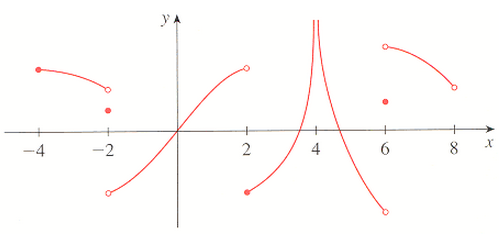
\includegraphics[height=3in]{Problem254}
      \end{center}

      \bigskip
      \begin{enumerate}
      \item 
        Write down the set of points where $f(x)$
        is continuous. (Use interval notation, with the union symbol $\cup$ if
        necessary). 

        \vskip1cm


        \ifthenelse{\boolean{answers}}{
          {\small          
            \hfill {\bf Answer:} $[-4, -2)\cup (-2, 2) \cup (2, 4) \cup (4, 6) \cup (6, 8)$ \phantom{XXXX}
          }} {
            \hfill {\bf Answer:}
            \underline{\phantom{XXXXXXXXXXXXXXXXXXXXXXXXXXXXX}}
          }

        \vskip1cm

      \item At how many points in the domain is the function discontinuous?

        \bigskip

        \ifthenelse{\boolean{answers}}{
          {\small          
            \hfill {\bf Answer:} \phantom{XXX} $4$ \phantom{XXXX}
            \vskip-2mm \hfill \underline{\phantom{XXXXXXX}}
        }} {
          \hfill {\bf Answer:} \underline{\phantom{XXXXXXX}}
        }
        \bigskip

      \item How many points in the domain are removable discontinuities?

        \bigskip

        \ifthenelse{\boolean{answers}}{
          {\small          
            \hfill {\bf Answer:} \phantom{XXX} $0$ \phantom{XXXX}
            \vskip-2mm \hfill \underline{\phantom{XXXXXXX}}
        }} {
          \hfill {\bf Answer:} \underline{\phantom{XXXXXXX}}
        }
        \bigskip


      \end{enumerate}

    \end{enumerate}
\end{document}


%%   \begin{tabular}{lllll}

%% \underline{\phantom{XX}} $(-\infty, -4]$ \phantom{XXX} &
%% \underline{\phantom{XX}} $(-\infty, -4)$ \phantom{XXX} &
%% \underline{\phantom{XX}} $(2, 4)$ \phantom{XXX} &
%% \underline{\phantom{XX}} $[2, 4]$\phantom{XXX} & \underline{\phantom{XX}} $(2, 6)$
%% \\[8pt]

%% \underline{\phantom{XX}} $[-4, -2]$ &
%% \underline{\phantom{XX}} $(-4, -2)$&
%% \underline{\phantom{XX}} $[4, 6]$&
%% \underline{\phantom{XX}} $(4, 6)$&
%% \underline{\phantom{XX}} $(8,\infty)$
%% \\[9pt]

%% \underline{\phantom{XX}} $[-2, 2]$&
%% \underline{\phantom{XX}} $(-2, 2)$&
%% \underline{\phantom{XX}} $(6,8)$&
%% \underline{\phantom{XX}} $[6,8)$&
%% \underline{\phantom{XX}} $[8,\infty)$

%%   \end{tabular}


\newpage
% 2.7.48
\item The quantity (in pounds) of a gourmet ground coffee that is sold by a
  coffee company at a price of $d$ dollars per pound is $Q = f(d)$.
  Circle the correct answer choices below.
  \begin{enumerate}[{\it i.}]
  \item 
    What is the meaning of the \emph{instantaneous rate of change} of $f(d)$
    at the point where $d=6$?
    \begin{enumerate}[(a)]
    \item 
      The rate of change of the price per pound with respect to the quantity of coffee
      sold when the price is \$6 per pound. 
    \item 
      The rate of change of the price per pound with respect to the quantity of
      coffee sold.
    \item 
      The supply of coffee needed to be sold to charge \$6 per pound.
    \item 
      The price of the coffee as a function of the supply.
    \item 
      The rate of change of the quantity of coffee sold with respect to the price
      per pound when the price is \$6 per pound.  
    \end{enumerate}
    % answer (a)
    \bigskip

  \item What are the units of the rate of change of $f(d)$?\\[4pt]
    (a) dollars \hfill (b) pounds/dollar  \hfill (c) pounds/(dollars/pound)
    \hfill (d) dollars/pound \\[4pt]
    (e) dollars/(pound/pound) \hskip1cm (f) pounds
    % answer: (c)
    \bigskip

  \item 
    In general, would you expect the rate of change of $f(d)$ at $d=6$ to be
    positive or negative?\\[4pt] 
    positive \hskip2cm negative    
  \end{enumerate}
  % answer: negative


